\section{Espais topològics 2AN i espais separables}

\begin{defi}
	Un espai topològic $X$ es diu que satisfà el segon axioma de numerabilitat (2AN) si té una base de cardinal numerable.
\end{defi}

\begin{example}
	Amb la topologia usual, $\real$ t\'e una base numerable: la fam\'ilia de tots els intervals oberts $(a, b)$ amb $a, b \in \q$. An\`alogament, també $\real^n$ té una base numerable:
	\[B=\left\{(a_1,b_1)\times\dots\times(a_n,b_n)\,|\,a_i, b_i\in \q, 1\leq i\leq n\right\}. \]
\end{example}

\begin{defi}
	Es diu que un conjunt $A$ és dens en $X$ si $\overline{A} = X$. Un espai s'anomena separable si té un subconjunt numerable dens.
\end{defi}

\begin{example}
	Tenim que $\overline{\q} = \real$. Com que $\q$ és numerable, $\real$ és separable. Més generalment, $\real^n$ és separable perquè admet $\q^n$ com a subconjunt dens.
\end{example}

\begin{prop}
	Un espai mètric $X$ és 2AN si i només si és separable.
\end{prop}
\begin{proof}
	Sigui $\B$ una base numerable de $X$. Per a cada $B \in \B$, prenem un punt $x_B \in B$ qualsevol. Llavors, com és fàcil de comprovar, el conjunt $\left\{x_B\right\}_{B \in \B}$ és dens.

	\quad

	Sigui $A$ un subconjunt numerable dens de l'espai. Llavors
	\[\B = \left\{B_{\sfrac{1}{n}} (a) \, | \, a\in A, \, n\in \n\right\}\]
	és una base numerable de l'espai. És numerable perquè és reunió numerable de conjunts numerables. A més, és una base ja que sigui $x$ un punt qualsevol i $U$ un entorn obert seu. Com que $x$ és interior a $U$, $\exists n>0$ tal que $B_{\sfrac{1}{n}}(x)\subset U$, llavors $B_{\sfrac{1}{2n}}(x)\cap A \neq \emptyset$ perquè $A$ és dens en $X$. Sigui $a \in B_{\sfrac{1}{2n}}(x)\cap A\subseteq U\cap A$, tenim que $x \in B_{\sfrac{1}{2n}}(a)$. Vegem que $B_{\sfrac{1}{2n}}(a)\subset U$. Sigui $y \in B_{\sfrac{1}{2n}}(a)$, per la desigualtat triangular es té
	\[d(x, y) \leq d(x, a) + d(a, y) < \frac{1}{2n} + \frac{1}{2n} = \frac{1}{n}\]
	i, per tant, $y\in B_{\sfrac{1}{n}}(x) \subset U \implies x \in B_{\sfrac{1}{2n}}(a)\subseteq B_{\sfrac{1}{n}}(x) \subset U$.
\end{proof}

\section{Topologia quocient}
\begin{obs}
	Siguin $X$ un conjunt i $\sim$ una relació d'equivalència, llavors $X/\sim$ \'es el conjunt de classes d'equivalència. Si $f\colon X\rightarrow Y$ exhaustiva, definim $x\sim x' \iff f(x) = f(x')$ i tenim que
	\begin{align*}
		\overline{f} \colon X/\sim &\rightarrow Y \\
		\left[ x \right] &\mapsto f(x)
	\end{align*}
	\'es bijectiva.
\end{obs}
\begin{defi}
	Sigui $X$ un espai topològic. Siguin $Y\subset X$ i $\pi \colon X \rightarrow Y$ exhaustiva. Diem que $Y$ t\'e la topologia quocient per $\pi$ si els oberts de $Y$ són
	\[ \T_Y = \left\{ V\subseteq Y\,|\,\pi^{-1}(V) \in \T_X \right\}. \]
\end{defi}
\begin{prop}
	Propietats:
	\begin{enumerate}
		\item La topologia quocient de $Y$ per $\pi$ \'es la m\'es fina que fa $\pi$ contínua.
		\item Sigui $g\circ\pi \colon X \stackrel{\pi}{\rightarrow} Y \stackrel{g}{\rightarrow} Z$. $g$ \'es contínua $\iff g\circ\pi$ \'es contínua.
	\end{enumerate}
\end{prop}
\begin{proof}
	Vegem-ho.
	\begin{enumerate}
		\item Immediat per la definició de topologia quocient.
		\item La implicació cap a la dreta: $g \circ \pi$ \'es contínua perquè \'es composició de contínues.

			La implicació cap a l'esquerra: Sigui $W \subseteq Z$ obert, $g^{-1}(W) \subseteq Y$ \'es obert ja que
			\[
				\left( g\circ \pi \right)^{-1}\left( W \right) \text{ obert} \implies \pi^{-1}\left( g^{-1}\left( W \right) \right) \text{obert} \implies g^{-1}\left( W \right) \text{ obert.}
			\]
	\end{enumerate}
\end{proof}
\begin{prop}[Tallar i enganxar]
	Siguin $f\colon X\rightarrow Y$ un homeomorfisme i $\sim_X$, $\sim_Y$ relacions d'equivalència a $X$ i a $Y$ tals que $x \sim_X x' \iff f\left( x \right) \sim_Y f\left( x' \right)$, llavors $f$ indueix un homeomorfisme $\overline{f} \colon X/\sim \rightarrow Y/\sim$.
\end{prop}
\begin{proof}
	Com que $x\sim x' \implies f\left( x \right) \sim f\left( x' \right)$, $f$ indueix una aplicació $\overline{f}\colon X/\sim \rightarrow Y/\sim$ que fa commutatiu el diagrama
	\[
		\begin{tikzcd}
			X\ar{r}{f}\ar{d}[swap]{p} & Y\ar{d}[swap]{q}\\[2ex]
			X/\sim \ar{r}{\overline{f}} & Y/\sim
		\end{tikzcd}
	\]
	Com que $q\circ f$ \'es contínua, per la propietat universal de la topologia quocient de $X/\sim$, $\overline{f}$ \'es contínua. Si $f$ \'es bijectiva, com que $x\sim x' \iff f\left( x \right) \sim f\left( x' \right)$, $\overline{f}$ \'es bijectiva. Apliquem el mateix raonament a $f^{-1}$ per deduir que $\overline{f}^{-1}$ \'es contínua.
\end{proof}
\begin{example}
	\begin{enumerate}
		\item[] 
		\item
			\[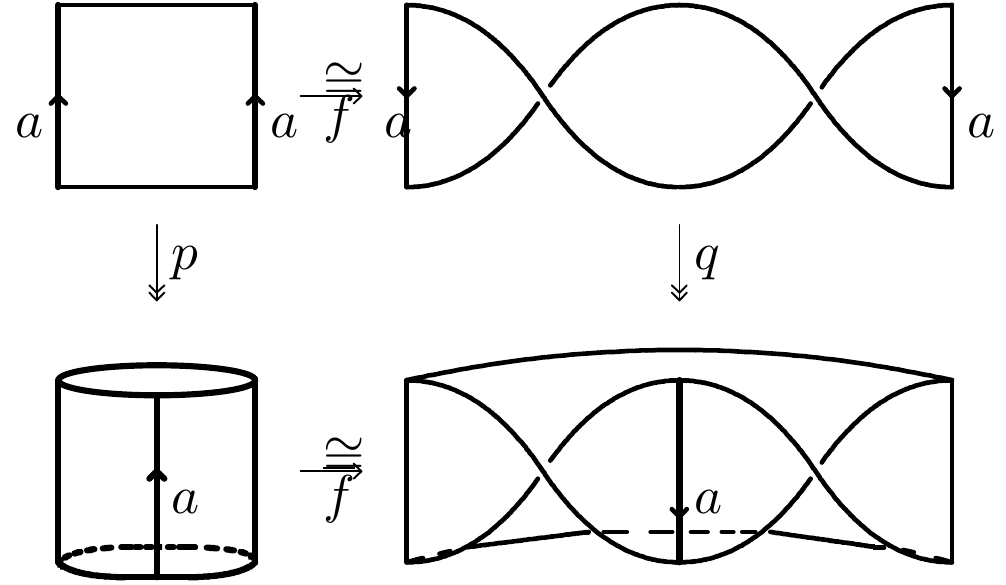
\includegraphics[scale=0.2]{figs_resum/cilindre.png}\]
		\item $\mathbb{D} = \left\{ \left( x, y \right) \,|\, x^2 + y^2 \leq 1 \right\}$
			\begin{multicols}{2}
				\[
					\begin{tikzcd}
						\mathbb{D}\ar{dr}\ar{d} & \\[2ex]
						\mathbb{D}/\sim \ar{r}{\cong} & \mathbb{S}^2
					\end{tikzcd}
				\]
				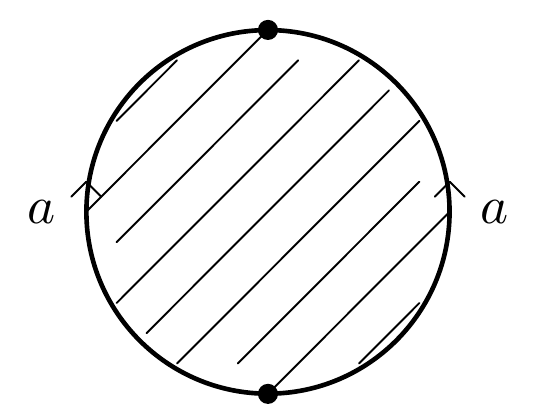
\includegraphics[scale=0.15]{figs_resum/esfera.png}
			\end{multicols}
		\item Altres: banda de Möbius, pla projectiu, ampolla de Klein, tor...
	\end{enumerate}
\end{example}

\section{Espai compacte i compacitat del producte}

\begin{defi}
	Un espai topològic $X$ és compacte si per tot recobriment obert $\mathcal{U}$ existeix un subrecobriment $\mathcal{V}\subset\mathcal{U}$ finit.
\end{defi}

\begin{lema}[Lema del tub]
	Siguin $X$ i $Y$ espais topològics, $Y$ compacte. Sigui $x\in X$ i $N$ obert de $X \times Y$ tal que $x\times Y \subset N$.
	Aleshores existeix $W \subset X$ obert tal que $x\times Y \subset W \times Y \subset N$.
\end{lema}
\begin{proof}
	Per cada punt $(x,y) \in x\times Y$ prenem un obert $U_y\times V_y$ de la base de $X\times Y$ que el contingui, de manera que $(U_y\times V_y) \subset N$. El conjunt de tots els $U_y\times V_y$ és un recobriment obert de $x\times Y$.

	$x \times Y \cong Y$ és compacte, del recobriment anterior se'n pot extraure un de finit $(U_1 \times V_1) \cup\dots\cup (U_n \times V_n)$.

	El conjunt $W = U_1 \cap\dots\cap U_n$ és obert de $X$ perquè és intersecció finita d'oberts, i $x \times Y \subset W\times Y \subset (U_1 \times V_1 \cup\dots\cup U_n \times V_n) \subset N$.
\end{proof}

\begin{prop}
	$X$, $Y$ espais topològics i $X \times Y$ la topologia producte. Aleshores
	\[X \times Y \text{ compacte } \Longleftrightarrow X,Y \text{ compactes}\]
\end{prop}
\begin{proof}
	Si $X \times Y$ és compacte i la projecció $\pi_X\!: X \times Y \rightarrow X$ és contínua, $\pi_X(X\times Y)=X$ és compacte. Anàlogament per $Y$.

	\quad

	Suposem que $X$ i $Y$ són compactes. Sigui $\mathcal{U}$ un recobriment obert de $X \times Y$. $x \times Y$ és compacte, per tant hi ha un recobriment finit $x \times Y \subset V_1 \cup\dots\cup V_n$ amb elements de $\mathcal{U}$.

	Considerem $N = V_1 \cup\dots\cup V_n$, pel lema del tub existeix un $x \in W \subset X$ tal que $x\times Y \subset W \times Y \subset N$. Per tant $V_1 \cup\dots\cup  V_n$ és un recobriment obert finit de $W \times Y$ amb elements de $\mathcal{U}$.

	Ara, per cada $x\in X$ apliquem el lema del tub i obtenim un $x \in W_x$ tal que $W_x \times Y$ té un recobriment finit amb elements de $\mathcal{U}$. Els $W_x$ formen un recobriment de $X$, i $X$ és compacte, tenim un recobriment finit $X = W_1 \cup\dots\cup W_n$. Per cada $W_i$ prenem els $V$ corresponents i obtenim un subrecobriment de $\mathcal{U}$ finit, per tant $X\times Y$ és compacte.

\end{proof}


\section{Tancats, Hausdorff i compacitat}

\begin{defi}
	Un espai topològic $X$ \'es Hausdorff si $\forall \: x, y \in X, \, \exists \: U,\, V$
	oberts tals que $U \cap V = \varnothing$ i $x \in U,\, y \in V$.
\end{defi}
\begin{prop}
	Tot supespai tancat d'un espai compacte \'es un espai compacte. 
\end{prop}
\begin{proof}
	Siguin $X$ un espai compacte, $Y \subseteq X$ un tancat i $\mathcal{U}$ un recobriment
	de $Y$ per oberts de $X$. Afegint l'obert $X \setminus Y$ obtenim un 
	recobriment obert de $X$ que, per ser $X$ compacte, cont\'e un 
	subrecobriment finit. Els oberts d'aquest subrecobriment diferents 
	de $X \setminus Y$  han de cobrir $Y$, i per tant formen un subrecobriment finit de 
	$\mathcal{U}$.
\end{proof}
\begin{example}
	La recta real amb la topologia de complements finits \'es un espai compacte i tamb\'e ho
	\'es qualsevol subespai d'aquesta, però nom\'es són tancats els conjunts finits de punts,
	d'on un subespai compacte pot no ser tancat.
\end{example}
\begin{prop}
	Tot subespai compacte d'un espai de Hausdorff \'es tancat.
\end{prop}
\begin{proof}
	Siguin $X$ un espai de Hausdorff i $Y \subseteq X$ un subconjunt compacte. Vegem que
	$X \setminus Y$ \'es obert comprovant que tot punt $x_0 \in X \setminus Y$ \'es interior. Com $X$
	\'es de Hausdorff, per a cada $y \in Y$ existeixen oberts disjunts $U_y, V_y$ tals
	que $x_0 \in U_y, y \in V_y$.

	La família $\{V_y\}_{y \in Y}$ forma un recobriment obert de $Y$. Per ser $Y$ compacte,
	cont\'e un subrecobriment finit $Y \subseteq V_{y_1} \cup \dots \cup V_{y_n}$.
	Considerem els oberts
	\[ 
		V = V_{y_1} \cup \dots \cup V_{y_n}, \,
		U = U_{y_1} \cap \dots \cap U_{y_n},
	\]
	que són disjunts ja que si $z \in V$, aleshores 
	existeix $y_i$ tal que $z \not\in U_{y_i}$,
	d'on $z \not\in U$. Per tant, $U \subseteq X \setminus Y$.
\end{proof}
\begin{prop}
	Sigui $f : X \longrightarrow Y$ una aplicació contínua i bijectiva. Si $X$ \'es compacte
	i $Y$ \'es de Hausdorff, aleshores $f$ \'es un homeomorfisme.
\end{prop}
\begin{proof}
	Hem de provar $f^{-1}$ \'es contínua, però això \'es equivalent a que $f$ sigui tancada. 
	Sigui $C$ un tancat de $X$. Com $X$ \'es compacte, $C$ tamb\'e ho \'es. Per ser imatge
	d'un compacte per una aplicació contínua, $f(C)$ \'es compacte i per la
	proposició anterior, com $Y$ \'es de Hausdorff, tamb\'e \'es tancat.
\end{proof}

\section{Espais connexos}

\begin{defi}
	Sigui $X$ un espai topològic. Una descomposició de $X$ consisteix en dos
	subconjunts $U, V \subseteq X$ no buits tals que
	\[
		X = U \cup V, \quad \overline{U} \cap V = \varnothing, \quad U \cap
		\overline{V} = \varnothing.
	\]
	Podem observar que $U$ i $V$ són tancats i oberts de $X$ i per tant
	donar una descomposició \'es equivalent a donar dos oberts disjunts no buits
	$U, V$ amb $X = U \cup V$.
\end{defi}

\begin{defi}
	Un espai topològic $X$ s'anomena connex si no admet cap descomposició, és
	a dir, no existeixen oberts disjunts $U, V \subseteq X$ no buits tals que
	$X = U \cup V$.
\end{defi}

\begin{defi}
	Sigui $X$ un espai topològic. Un camí de $X$ \'es una aplicació contínua
	$\sigma : I = [0, 1] \longrightarrow X$.
\end{defi}

\begin{defi}
	Un espai topològic $X$ s'anomena arc-connex si per a tot parell de punts
	$x, y \in X$ existeix un camí $\sigma: I \longrightarrow X$ tal que $\sigma(0)
	= x$ i $\sigma(1) = y$.
\end{defi}

\begin{example}
	Hi ha espais connexos que no són arc-connexos. Per construir-ne un exemple
	considerem el subconjunt de $\R^2$
	\[ 
		C = \lp[0, 1] \times \{0\}\rp \cup \lp 
		\bigcup \limits_{n \in \n} \lp \lc  \frac{1}{n} \rc 
		\times [0, 1] \rp \rp \cup \lp 0, 1\rp
	\]
	que s'anomena ``la pinta i la puça``.
\end{example}
\begin{prop}
	Sigui $X$ un espai topològic tal que per tota $x \in X$ existeix $x \in U$
	obert arc-connex. Aleshores 
	\[X \text{ connex} \iff X \text{ arc-connex}\]
\end{prop}

\begin{proof}
	La implicació conversa \'es una propietat dels espais arc-connexos en general.
	Vegem ara la implicació directa. Sigui $C$ el component maximal arc-connex 
	que conté $x$. Com $\forall \: y \in C$ existeix un obert arc-connex $y \in
	U$, per ser $C$ maximal $y \in U \subseteq C$ i $C$ \'es obert. Si $C$
	és l'únic component arc-connex aleshores $C = X$ i per tant $X$ és arc-connex.
	En cas contrari, $X$ és la unió disjunta de components arc-connexos, per tant
	$C = X \setminus \bigcup D$, on $D$ són els altres components arc-connexos.
	Com hem vist, aquests són oberts i per tant $C$ és tancat. Com $C$ és tancat
	i obert $C \neq \varnothing$ i $X$ és connex, $C = X$ i per tant $X$ és
	arc-connex.
\end{proof}
\section{Índexs}
\iffalse
	\begin{obs}
		No cal saber les demostracions dels teoremes de Poincaré-Bohl i de no retracció (per l'examen, per la vida sí).
	\end{obs}
\fi
\begin{teo*}[Invariància de l'índex per homotopies]
    Siguin $f, g \colon \mathbb{S}^1 \to \real ^2$ corbes tancades i sigui $p\in \real^2 \setminus \lp f\lp \mathbb{S}^1\rp \cup g\lp \mathbb{S}^1\rp\rp$. Aleshores,
    \[
        \mu \lp f, p\rp = \mu\lp g, p \rp \iff f \simeq g  \colon \mathbb{S}^1 \to \real \setminus \lc p \rc.
    \]
\end{teo*}

\iffalse
	\begin{teo*}[Poincaré-Bohl]
		Siguin $f, g \colon \mathbb{S}^1 \to \real ^2 \setminus \lc p \rc$ corbes tancades tals que $p \notin \overline{f\lp z \rp g \lp z \rp}, \, \forall z \in \mathbb{S}^1$. Aleshores,
		\[
			\mu \lp f, p\rp = \mu\lp g, p \rp.
		\]

	\end{teo*}
	\begin{proof}
		Recordatori: aquesta demostració no entra a l'examen. Vegem que $f \simeq g \colon \mathbb{S}^1 \to \real ^2 \setminus \lc p \rc$. En virtut del teorema d'invariància de l'índex per homotopies, basta observar que l'apliació
		\begin{align*}
			H \colon \mathbb{S}^1 &\to \real ^2 \setminus \lc p \rc \\
			\lp z, t \rp &\mapsto \lp 1-t \rp f\lp z \rp + tg\lp z \rp
		\end{align*}
		és una homotopia d'$f$ a $g$ en $\real^2 \setminus \lc p \rc$.
	\end{proof}
\fi

\begin{teo*}[Rouché]
    Siguin $f, g \colon \mathbb{S}^1 \to \real ^2 \setminus \lc p \rc$ corbes tancades. Aleshores,
    \[
        d \lp f \lp z \rp, g \lp z \rp \rp < d \lp f \lp z \rp, p \rp, \, \forall z\in \mathbb{S}^1 \implies \mu \lp f, p\rp = \mu\lp g, p \rp.
    \]
    
\end{teo*}
\begin{proof}
    \[
        d \lp f \lp z \rp, g \lp z \rp \rp < d \lp f \lp z \rp, p \rp \implies p \notin \overline{f\lp z \rp g \lp z \rp} \stackrel{\text{P-B}}{\implies} \mu \lp f, p\rp = \mu\lp g, p \rp.
    \]
\end{proof}
\begin{teo*}[Bolzano (dim 2)]
	Sigui $F\colon \mathbb{D} \to \real ^2$ contínua, on $\mathbb{D}$ és el disc unitat tancat. Sigui $f=F_{|\mathbb{S}^1}$ i sigui $P \in \real ^2$. Aleshores,
	\[
		\mu\lp f, P \rp \neq 0 \implies \exists Q \in \mathbb{D} \tq F\lp Q \rp = P.
	\]
\end{teo*}

\begin{proof}
	Suposem que $\mu\lp f, P \rp \neq 0$ i que $\nexists Q \in \mathbb{D} \tq F\lp Q\rp = P$.
	\[
		\begin{array}{lclcl}
			\mathbb{S}^1 \times I & \stackrel{\pi}{\to} & \mathbb{D} & \stackrel{F}{\to} & \real ^2 \setminus \lc P \rc \\
			\lp z, t \rp & \mapsto & zt & \mapsto & F\lp zt \rp \\
			\lp z, 0 \rp & \mapsto & 0 & \mapsto & F\lp 0 \rp\\
			\lp z, 1 \rp & \mapsto & z & \mapsto & F\lp z \rp = f\lp z \rp
		\end{array}
	\]
	Tenim, doncs, que $F \circ \pi$ és una homotopia entre $f$ i la funció constant zero. Finalment, pel teorema d'invariància de l'índex d'homotopies, tenim que $\mu \lp f, P \rp = 0$ i hem incoregut en una contradicció.
\end{proof}

\iffalse
	\begin{defi}
		Siguin $X$ un espai topològic i $A\subseteq X$. Una retracció d'$X$ en $A$ és una aplicació contínua $r\colon X \to A$ tal que $r_{|A}=\Id_A$.
	\end{defi}

	\begin{teo*}[No retracció]
		No existeix cap retracció de $\mathbb{D}$ a $\mathbb{S}^1$.
	\end{teo*}

	\begin{proof}
		Recordatori: aquesta demostració no entra a l'examen.
		Suposem que $r\colon \mathbb{D} \to \mathbb{S}^1$ és una retracció. Com que $r_{|\mathbb{S}^1} $ és la identitat, tenim
		\[
			\mu\lp r_{|\mathbb{S}^1}, 0\rp=1.
		\]
		Finalment, perl teorema de Bolzano, tenim que $\exists x \in \mathbb{D} \tq r\lp x\rp=0$, la qual cosa és una contradicció.
	\end{proof}
\fi

\begin{teo*}[Punt fix de Brouwer]
	Sigui $\mathbb{B}\subset \real ^n$ la bola tancada unitat de centre $0$ i sigui $f\colon \mathbb{B} \to \mathbb{B}$ contínua. Aleshores, $f$ té un punt fix.
\end{teo*}

\begin{proof}
	Només demostrarem el cas $n=2$. Suposem que $f$ no té cap punt fix. Definim $g\colon \mathbb{D} \to \mathbb{S}^1$, de manera que $g\lp x \rp$ és la intersecció de la semirecta amb origen $f\lp x \rp$ que passa per $x$ amb $\mathbb{S}^1$. Vegem que $g$ és contínua. Tenim que
	\[
		g\lp x \rp = x+\lambda\frac{x-f\lp x \rp}{\norm{x-f\lp x \rp}}, \qquad \lambda \geq 0.
	\]
	Com que $g\lp x\rp \in \mathbb{S}^1$, podem imposar $\norm{g\lp x \rp}^2 = 1$
	\begin{align*}
		\norm{g\lp x \rp}^2 &= \left< x+\lambda\frac{x-f\lp x \rp}{\norm{x-f\lp x \rp}}, x+\lambda\frac{x-f\lp x \rp}{\norm{x-f\lp x \rp}} \right> = \\
		&=  \left< x, x \right> + 2\left< x, \lambda\frac{x-f\lp x \rp}{\norm{x-f\lp x \rp}} \right> + \left<\lambda\frac{x-f\lp x \rp}{\norm{x-f\lp x \rp}}, \lambda\frac{x-f\lp x \rp}{\norm{x-f\lp x \rp}} \right> = \\
		&=  \left< x, x \right> + 2\lambda \left< x, \frac{x-f\lp x \rp}{\norm{x-f\lp x \rp}} \right> + \lambda ^2 = 1.
	\end{align*}
	Ara, aïllem $\lambda$ i ens quedem amb la solució positiva
	\begin{align*}
		\lambda &= \frac{-2\left< x, \frac{x-f\lp x \rp}{\norm{x-f\lp x \rp}} \right> + \sqrt{4\left< x, \frac{x-f\lp x \rp}{\norm{x-f\lp x \rp}} \right> ^2 -4\lp \left<x, x\right> -1 \rp}}{2} = \\
		&= -\left< x, \frac{x-f\lp x \rp}{\norm{x-f\lp x \rp}} \right> + \sqrt{1+\left< x, \frac{x-f\lp x \rp}{\norm{x-f\lp x \rp}} \right> ^2 -\left<x, x\right>}.
	\end{align*}
	L'expressió que ens dóna $\lambda$ és contínua i, per tant, $g$ també ho és. Però aleshores $g$ és una retracció i incorrem en una contradicció amb el teorema de no retracció.
\end{proof}

\section{Superfícies}

\begin{defi}[Varietat]
	Sigui $M$ un espai topològic. Direm que $M$ és una varietat de dimensió $n$ si:
	\begin{enumerate}[i)]
	\item $M$ és Hausdorff
	\item $M$ és $2AN$
	\item $\forall x \in M$, $\exists U \ni x$ obert i un homeomorfisme
		$\phi \colon U \to \real^n$ ($M$ localment homeomorf a $\real^n$)
\end{enumerate}
\end{defi}

\begin{example}
	\begin{enumerate}
		\item[]
		\item $n = 1$, són corbes, per exemple $\real$ o $\mathbb{S}$. Més en general:
			\begin{itemize}
				\item No s'admeten autointerseccions
				\item No podem afegir límits (extrems) a les corbes.
			\end{itemize}
		\item $n = 2$, són superfícies.
	    % TODO poner pantallaso rico papi
		\item Que $M$ hagi de ser Hausdorff i $2AN$ és per evitar patologies (com els punts
			dobles) i a més ens permet triangular
		\item Superfícies poligonals: $\mathbb{T}$, $\mathbb{K}$ (són compactes i convexes)
		\item Superfícies estàndard: superfícies poligonals corresponents a les paraules.
	\end{enumerate}
\end{example}

\begin{teo*}[C]
	Tota superfície $S$ compacta i connexa és homeomorfa a una única superfície estàndard.
	\begin{itemize}
		\item $A_0 \colon aa^{-1} (g = 0) \rightarrow A_0 \cong \mathbb{S}^2$
		\item $A_g \colon a_1b_1a^{-1}_1 b^{-1}_1 \cdots a_gb_ga^{-1}_gb^{-1}_g (g \geq 1)
			\rightarrow A_g \cong g \mathbb{T}$ ($g$-tors)
		\item $B_g \colon a_1a_1 \cdots a_ga_g (g \geq 1) \rightarrow B_g \cong g \mathbb{P}^2$
			($g$-plans projectius)
	\end{itemize}
	($g$ és el gènere de la superfície)
\end{teo*}

\begin{defi}[Orientabilitat]
	$S$ és no orientable si conté una cinta de Möbius. $S$ és orientable en cas contrari.
\end{defi}

\begin{example}
	\begin{enumerate}
		\item[]
		\item $g \Po^2$, $g \geq 1$ no és orientable.
		\item $g \mathbb{T}^2$, $g \geq 0$ sí que és orientable. ($g = 0$, $A_0 \leadsto \mathbb{S}^2$)
		\item $S \cong S^\prime \implies $ tenen la mateixa orientabilitat. De fet, dues superfícies
			són homeomorfes si tenen el mateix gènere i la mateixa orientabilitat.
	\end{enumerate}
\end{example}

\begin{defi}[Característica d'Euler]
	Sigui $(S, T)$ una superfície triangulada, definim la característica d'Euler de $T$ per
	\[
		\chi (s, t) = v - a + c
	\]
	On $v$ són els vèrtex, $a$ les arestes i $c$ les cares.
\end{defi}

\begin{teo*}
	$\chi(S)$ és independent de la triangulació.
\end{teo*}

\begin{example}
	\begin{enumerate}
		\item[]
		\item $\chi(\text{poligonal}) = \cdots = 1 + v^\prime - n$. Amb $v^\prime$, \# de punts que són
			imatge dels vèrtexs del poligon.
		\item
			\[
				\begin{aligned}
					\chi (\text{estàndard}) \colon \quad & \chi(A_0) = 2 \\ & \chi \left( g \mathbb{T}^2 \right) = 2 -2g \\
					& \chi \left( g\Po^2 \right) = 2 - g 
				\end{aligned}
			\]
	\end{enumerate}
\end{example}

\begin{defi}[Suma connexa de superfícies]
	Siguin $S, S^\prime$ superfícies, $D \subset S$, $D^\prime \subset S^\prime$ discs tancats i
	$h \colon \partial D \to \partial D^\prime$ homeomorfisme llavors
	\[
		S \# S^\prime = \frac{\left(S \setminus \mathring{D} \right) \cup 
		\left( S^\prime \setminus \mathring{D^\prime} \right)}{h \colon \partial D \to \partial D^\prime}
	\]
\end{defi}
